\documentclass[12pt] {article}

%%% Preambuła %%%
\usepackage[T1]{fontenc}
\usepackage[polish]{babel}
\usepackage[utf8]{inputenc}
\usepackage{lmodern}
\usepackage{hyperref}
\usepackage{mathptmx}
\usepackage{float}
\usepackage{graphicx}
\usepackage{xcolor}
\selectlanguage{polish}
\usepackage{titlesec}


%%% Strona tytułowa %%%
\title 
{	
	
\includegraphics[scale = 1]{res/Logo} \\
	{
		\normalfont\sffamily
		Aplikacja webowa do zarządzania serwerem DNS \\[0.1in]
		Dokumentacja użytkownika\\ [0.1in]
		\large 
		Inżynieria Oprogramowania \\
		Wydział Fizyki i Informatyki Stosowanej \\
		Informatyka Stosowana, 3 rok \\
	}
}

\author 
{\normalfont\sffamily Arkadiusz Kasprzak \and \normalfont\sffamily Jarosław Cierpich \and \normalfont\sffamily Jakub Kowalski \and \normalfont\sffamily Konrad Pasik \and \normalfont\sffamily Krystian Molenda}
\date{}


\titleformat{\section}
  {\normalfont\sffamily\Large\bfseries\color{orange}}
  {\thesection}{1em}{}
	
\definecolor{ao}{rgb}{0.0, 0.0, 1.0}	
\definecolor{forestgreen(web)}{rgb}{0.13, 0.55, 0.13}

\begin{document}


%%% Strona tytułowa %%%
\maketitle
\newpage

%%% Spis treści %%%
\tableofcontents

\newpage 

\section{Instalacja}
Aplikacja będzie dostarczana w postaci \textit{fat JAR} zatem wszystkie potrzebne biblioteki będą dołączone. Oprócz samej aplikacji do działania będą wymagane:
\begin{itemize}
\item Java w wersji 8
\item Baza danych PostgreSQL 11
\item Aplikacja pgAdmin 4
\end{itemize}
W celu uruchomienia aplikacji należy wykonać załączony skrypt w zależności od systemu operacyjnego: Linux - skrypt .sh, Windows - plik .bat. 

\section{Konfiguracja}
Konfigurację aplikacji można zmieniać na dwa sposoby:
\begin{itemize}
\item przy uruchomieniu aplikacji za pomocą dedykowanego graficznego interfejsu użytkownika, gdzie można zdefiniować takie parametry jak:
\begin{itemize}
\item parametry bazy: login, hasło, adres ip, numer portu, nazwa bazy danych
\item ścieżka do aplikacji pgAdmin
\item ścieżka zapisu plików kopii zapasowej bazy danych
\end{itemize}
\item edytując wygenerowany plik .yaml, gdzie zapisane są wszystkie parametry podane wcześniej poprzez graficzny interfejs użytkownika
\end{itemize}
Graficzny interfejs użytkownika można ponownie uruchomić usuwając plik .yaml i restartując aplikację.\newline
Zakładanie konta administracyjnego odbywa się dokładnie tam samo jak zakładanie zwykłego konta, tj. za pomocą formularza rejestracyjnego na stronie. Pierwszy zarejestrowany użytkownik dostaje dostęp do systemu. Każdy następny zarejestrowany użytkownik musi zostać zatwierdzony przez zweryfikowane konto.

\newpage
\section{Przewodnik użytkownika}
W celu korzystania z systemu należy zarejestrować użytkownika za pomocą formularza:
\begin{figure}[H]
\centering
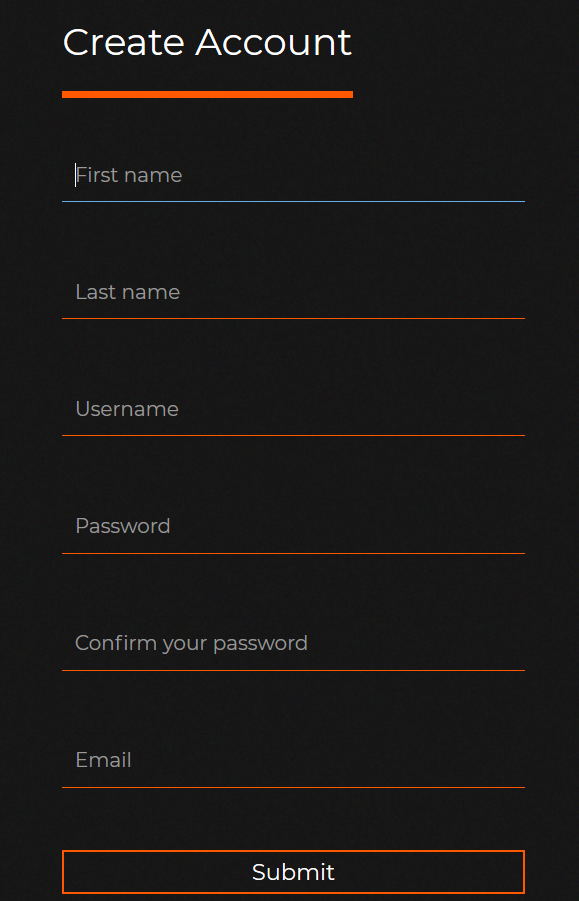
\includegraphics[scale=0.4]{res/Rejestracja}
\end{figure}
Pierwsze utworzone konto jest automatycznie weryfikowane. Każde następne musi zostać zweryfikowane przez już zatwierdzonego użytkownika. \newpage
Następnie należy się zalogować:
\begin{figure}[H]
\centering
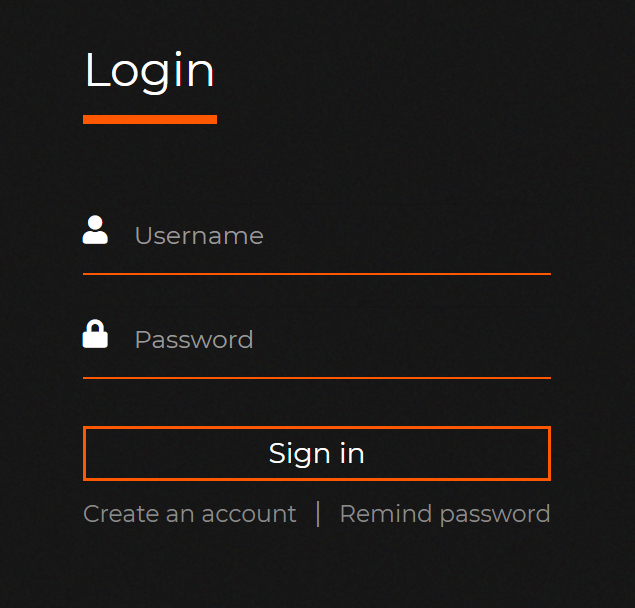
\includegraphics[scale=0.4]{res/Login_1}
\end{figure}
Po zalogowaniu się wszystkie możliwe akcje są przedstawione na stronie głównej:
\begin{figure}[H]
\centering
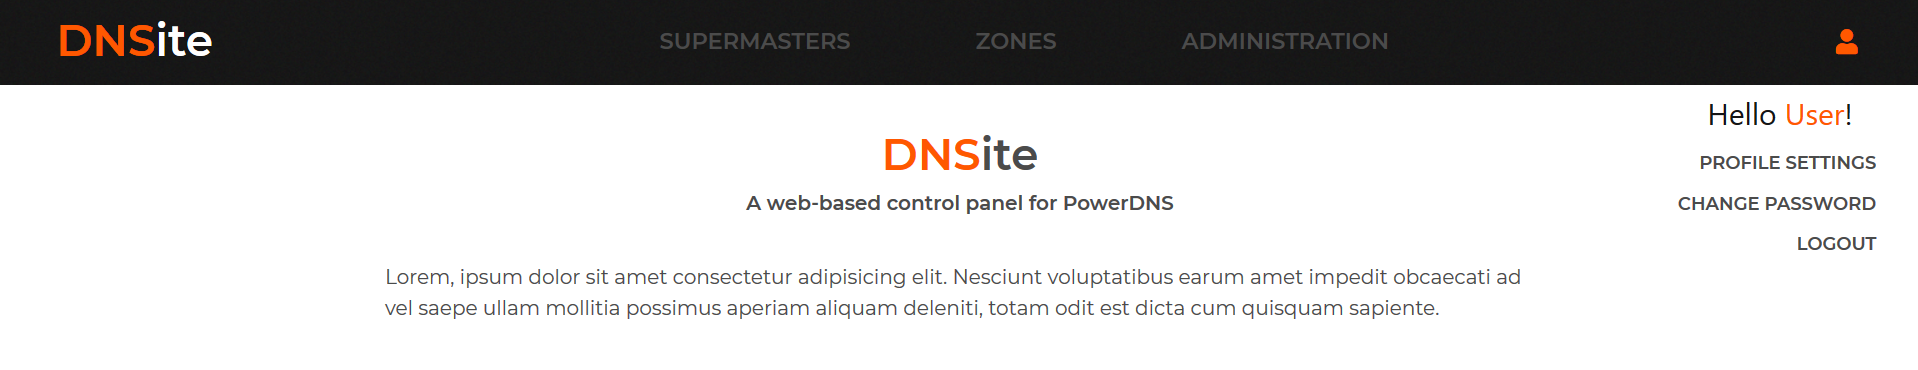
\includegraphics[width=\textwidth]{res/Glowna_strona}
\end{figure}
Po prawej stronie znajduje się ikona \textit{użytkownika}. Po wciśnięciu ikony pojawia się menu zarządzania kontem. Dodatkowo panel nawigacyjny posiada odnośniki do widoków pozwalających na wszelkie potrzebne operacje na zasobach serwera DNS.\newline
*Zrzut ekranu strony głównej został wykonany na wersji produkcyjnej. Zostanie zaktualizowany po zakończeniu procesu dewelopmentu. \newpage
Interfejs graficzny służący do wprowadzania zmian w postaci tabelki:
\begin{figure}[H]
\centering
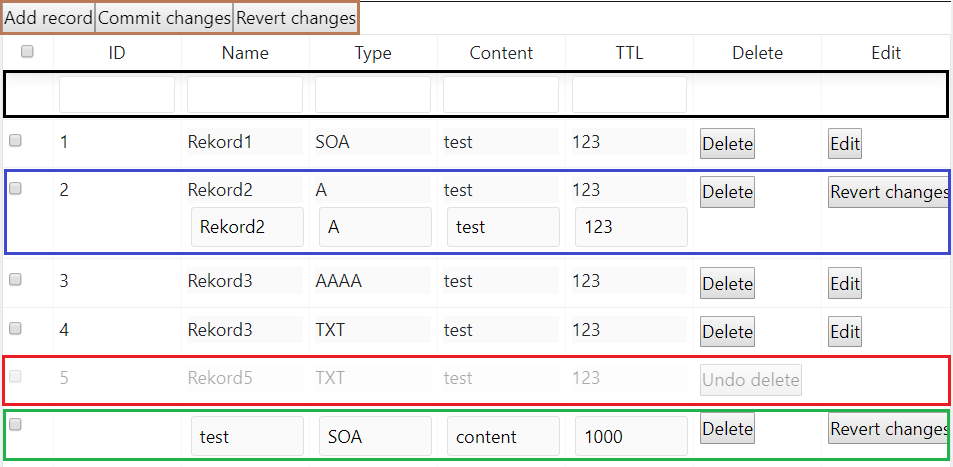
\includegraphics[width=\textwidth]{res/Tabelka}
\end{figure}


Możliwe operacje:
\begin{itemize}
\item \color{brown} Menu główne: 
\begin{itemize}
\item Dodanie nowego rekordu.
\item Zaaplikowanie wszystkim zmian i zaktualizowanie bazy danych
\item Powrót do stanu początkowego (wszystkie zmiany wprowadzone w trakcie sesji)
\end{itemize} \color{black}
\item \color{black} filtrowanie wyników \color{black}
\item \color{ao} edytowanie rekordu \color{black}
\item \color{red} usuwanie rekordu \color{black}
\item \color{forestgreen(web)} nowy wpis w tabelce - kontekst do dodania nowego rekordu \color{black}
\item Wprowadzenie zmian do wszystkich zaznaczonych i oznaczonych jako aktualnie edytowanych rekordów (niewidoczne na zrzucie ekranu)
\end{itemize}

Ważne informacje:
\begin{itemize}
\item Pola, gdzie mamy wybór spośród pewnej puli możliwości będą definiowane jako lista opcji (wybór jednej z możliwości)
\item Niektóre pola, np.: notified serial są tylko informacyjne i nie można ich zmieniać
\item Wszystkie widoki do edytowania są w formie tabelki, jedynym wyjątkiem są domeny, gdzie oprócz możliwości edytowania za pomocą listy jest również możliwość edytowania za pomocą formularza. 
\begin{figure}[H]
\centering
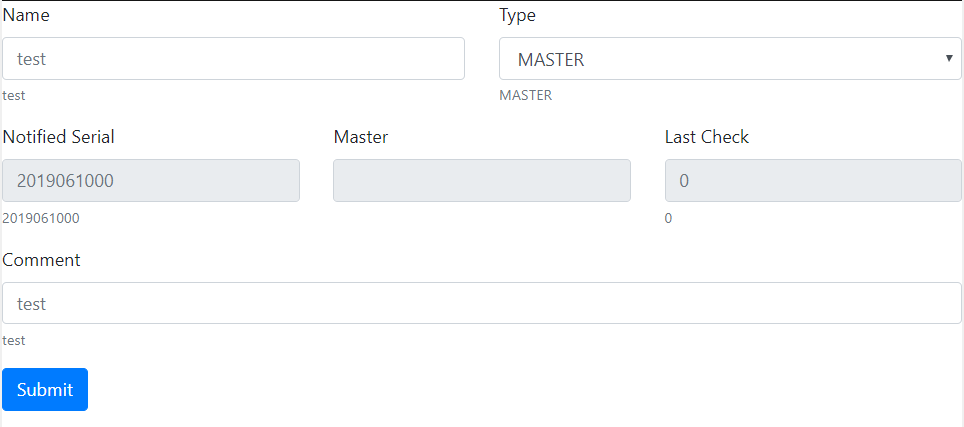
\includegraphics[width=\textwidth]{res/formularz}
\end{figure}
\end{itemize}

\end{document}